\documentclass{beamer}

\input{preamble}
\definecolor{darkgreen}{RGB}{20,150,50}
\definecolor{Periwinkle}{rgb}{0.0, 0.0, 0.0}
\usepackage{listings}
\usepackage{amsmath,bm}
\newcommand{\book}{\includegraphics[width=10pt]{img/proceeding-logo.jpg}}
\newcommand{\github}{\includegraphics[width=10pt]{img/github-logo.jpg}}
\begin{document}

\begin{frame}
  \titlepage
\end{frame}


\begin{frame}{Motivations}

\structure{Neural state-space models}  are widely used for dynamical systems. We have also applied them to the \href{https://www.nonlinearbenchmark.org/}{nonlinear benchmarks}!
  	\begin{itemize}
	\item[\book]
		\begin{tiny}
	\structure{M. Forgione and D.Piga.}
    Continuous-time system identification with neural networks: model structures and \vskip -1em
    fitting 
    criteria. \emph{European Journal of Control, 2021}
		\end{tiny}\\								

 	\item[\book]
		\begin{tiny}
	\structure{B. Mavkov, M. Forgione and D.Piga.}
									Integrated Neural Networks for Nonlinear Continuous-Time System \vskip -1em Identification.
									\textcolor{Periwinkle}{\textit{IEEE Control Systems Letters, 4(4), pp 851-856, 
2020.}}
		\end{tiny}\\								
% 	\item[\book]
% 		\begin{tiny}
% 	\structure{M. Forgione and D.Piga.}
% 				Model structures and fitting criteria for system identification with neural networks.
% 				%\vskip -1em
% 				\textcolor{Periwinkle}{\textit{In Proc. of the 14th. IEEE Application of Information and Communication Technologies Conference (AICT), \vskip -1em 2020}}
% 		\end{tiny}\\
	\item[\book]
		\begin{tiny}
	\structure{G. Beintema, R. Toth, and M. Schoukens.}
				Nonlinear state-space identification using deep encoder networks.\\
				\vskip -1em
				\textcolor{Periwinkle}{\textit{In Proc. of the 13rd Conference on Learning for Dynamics and Control, (PMLR), 2021.}}
		\end{tiny}\\
	\end{itemize}

\vskip 1em
\pause

Little focus so far on \structure{uncertainty quantification}.
\begin{itemize}
\item What's our confidence in the model predictions?
\item Can we detect model usage outside its validity range?
%\item %We show results on a (synthetic) Wiener-Hammerstein benchmark. 
\end{itemize}

% \begin{itemize}
% \item We formalizeHow confident;
% \item We developed basic uncertainty quantification techniques; 
% \item We show results on a (synthetic) Wiener-Hammerstein benchmark. 
% \end{itemize}

\vskip 1.0 em
\pause
 	\begin{itemize}
	\item[\book]
		\begin{tiny}
	\structure{M.~Forgione and D.~Piga.}
    Neural state-space models: Empirical evaluation of uncertainty quantification. \vskip -1em
    \emph{Accepted for presentation at the 22nd IFAC World Congress, 2023}
		\end{tiny}\\
      \item[\github]\begin{tiny}{\url{https://github.com/forgi86/sysid-neural-unc}}\end{tiny}
	\end{itemize}
	
\end{frame}

\begin{frame}{Settings}
The \structure{true system} is assumed to have a state-space representation:
\begin{equation*}
\begin{split}
 x^+ &= f(x, u) \\
 y^{\text o}  &= g(x),\\
\end{split}
\end{equation*}
with noisy discrete-time measurements available: $y = y^{\text o} + e$.
\pause
\vskip 1em
\structure{Training dataset} $\Did$: a single input/output sequence with:
\begin{itemize}
\item input samples $\tvec{u} = \{u_{1},\;u_{1},\dots,\;u_{\nsamp}\}$
\item output samples  $\tvec{y} = \{y_{1},\;y_{1},\dots,\;y_{\nsamp}\}$ 
\end{itemize}
\vskip 1em
\pause
\structure{Objective}: estimate a model of the system.
\vskip 1em
\pause
Note: output error model considered here (no process noise). 
%The case of process noise is much harder...% may be dealt with tools like ExpecaM, variational inference, MCMC, ...)
\end{frame}


\begin{frame}{Neural state-space models}{}
A very \structure{generic} neural model structure:
%\begin{align*}
% x_{k+1} &= \NN_f(x, u;\;\theta)\\
%    y_k  &= \NN_u(x; \theta)
%\end{align*}
\begin{align*}
 {x}^+ &= \NN_f(x, u;\;\theta)\\
    y  &= \NN_g(x; \theta)
\end{align*}

where $\NN_f$, $\NN_g$ are feed-forward neural networks, e.g.:
\begin{align*} 
\NN(z) &= W_2 \sigma \left(W_1z + b_1\right) + b_2 \\
\theta &= \text{vec}(W_1, b_1, W_2, b_2)\\
\sigma(\cdot) & \text{  static non-linearity}
\end{align*}
\vskip .5em\
\pause
Can be  \structure{specialized}, according to available system knowledge:
\begin{itemize}
  \item State fully observed $\Rightarrow$ 
  \begin{align*}
  x^+ &= \NN_f(x, u;\;\theta)\\
    y  &= x
\end{align*}
%   \pause
%  \item Linear approximation available $\Rightarrow$
% \begin{equation*}
% \begin{split}
%  \dot x &= A x + B u + \NN_f(x_{k}, u_{k}; \theta)\\
%  y     &= C x + \NN_g(x, u; \theta)
%  \end{split}
% \end{equation*}
\item ...
 \end{itemize}
\end{frame}

\begin{frame}{Neural state-space models}{Physics-inspired model structures}
%\vskip 1em
 Two-tank system. Input: flow $u$ in upper tank, output: lower tank level $x_2$.
 \begin{columns}
  \column{.6\textwidth}
  \begin{itemize}
   \item The system has two states: $x_1$ and $x_2$
   \item State $x_1$ does not depend on $x_2$
   \item State $x_2$ does not depend directly on $u$
   \item The state $x_2$ is measured
   \end{itemize}
  \column{.3\textwidth}
  \begin{center}
  \includegraphics[width=.6\textwidth]{img/CTS/CTS_scheme.pdf}
  \end{center}
\end{columns}
 %\pause
 \vskip 2em
 These observations are embedded in the \structure{physics-inspired} neural model:
% \begin{columns}
% \column{.5\textwidth}
\vskip -1.5em
\begin{small}
 \begin{align*}
  \dot x_1 &= \mathcal{N}_{1}(x_1, u;\;\theta)\\
  \dot x_2 &= \mathcal{N}_{2}(x_1, x_2;\;\theta)\\
  y        &= x_2
 \end{align*}
\end{small}
%  \column{.5\textwidth}
\vskip 0em

 	\begin{itemize}
	\item[\book]
		\begin{tiny}
	\structure{M. Forgione and D.Piga.}
    Continuous-time system identification with neural networks: model structures and \vskip -1em
    fitting 
    criteria. \emph{European Journal of Control, 2021}
		\end{tiny}\\								
  \end{itemize}
\end{frame}
% 
% \begin{frame}{Training Neural Dynamical Models}
% % The \structure{naive} 1-step prediction is constructed through 
%  In principle, \structure{simulation error minimization} is a valid strategy:
%  \begin{equation*}
%   \theta^o = \arg \min_{\theta, x_0} \sum_{k=0}^{\nsamp-1} \norm{\hat y_k^\mathrm{sim}(\theta, x_0) - y_k}^2
%  \end{equation*}
%  where
%  \begin{equation*}
%  \begin{split}
%   x_{k+1}^{\rm sim} &= \NN_f(x_k^{\rm sim}, u_k;\;\theta)\\
%   \hat{y}_k^{\rm sim} &= \NN_g(x_k;\;\theta)
%   \end{split}
%  \end{equation*}
%  for $k=0,1,\dots,\nsamp-1$.\\
% \pause
% \vskip .5em
%  However, it is not convenient from a computational perspective:
%  \begin{itemize}
%   \item Simulation is not parallelizable. Several neural network evaluations have to be performed \structure{sequentially}.
%   \item \structure{Back-propagation cost} increases with the sequence length
%  \end{itemize}
%  \pause
%  \vskip .5em
%  We minimize instead the simulation error over \structure{batches} of $\batchsize$  \structure{subsequences}, each one of length $\seqlen \ll N$.
% \end{frame}



\begin{frame}{Bayesian Framework}{}
We can frame model learning problem in a Bayesian framework:
\begin{align*}
    x^+ &=  \mathcal{N}_f(x, u; \theta)\\
    \hat y   &= \mathcal{N}_g(x; \theta)\\
    y &= \hat y + e\\
    \theta &\sim \mathcal{N}\left(0, \sigma^2_\theta\right),\;\; e \sim \mathcal{N}\left(0, \sigma^2_e\right)
\end{align*}
\pause
Then, there exist the \structure{posterior} of $\theta$ given observed data $\mathcal{D} = \{\tvec{u}, \tvec{y} \}$ \dots
\begin{equation*}
 p(\theta | \mathcal{D}) = \frac{p(\mathcal{D}|\theta) p(\theta)}{\alert{p(\mathcal{D})}},
\end{equation*}
\pause
\dots and the posterior on a new sequence $\tvec{y}^*$, given input sequence $\tvec{u}^*$:
\begin{equation*}
 p(\tvec{y}^* | \tvec{u}^*, \mathcal{D}) = \int_{\alert{\theta \in \Theta}} p(\tvec{y}^* | \tvec{u}^*, \theta) p(\theta | \mathcal{D})\; d\theta
\end{equation*}
\end{frame}

\begin{frame}{Challenges}
\begin{itemize}
 \item What are good Bayesian models structures (architecture + priors)?
  \begin{itemize}
  \item What \structure{families} of dynamical systems are likely under given assumptions?
  \end{itemize}
 \vskip 1em
 \pause
 \item How to obtain  the posterior parameter distribution $p(\theta | \mathcal{D})$ and of the posterior predictive distribution 
 $p(\tvec{y}^* | \tvec{u}^*, \mathcal{D})$?% is extremely hard.
 \begin{itemize}
 \item $p(\theta | \mathcal{D}) = \frac{p(\mathcal{D}|\theta) p(\theta)}{\alert{p(\mathcal{D})}}$ is accessible up to the denominator constant.
 \item $
 p(\tvec{y}^* | \tvec{u}^*, \mathcal{D}) = \int_{\alert{\theta \in \Theta}} p(\tvec{y}^* | \tvec{u}^*, \theta) p(\theta | \mathcal{D})\; d\theta
$ is a hard multi-dimensional integral anyway...
 \end{itemize}
 \end{itemize}
 \vskip 2em
 \pause  
 In this preliminary contribution we do not provide an answer to 1  and use the simplest approach to tackle 2: Laplace approximation + linearization.
\end{frame} 


\begin{frame}{Laplace approximation}
\structure{Quadratic} approximation of the (negative) log-posterior around a \emph{mode}, leading to a \structure{Gaussian} parameter posterior approximation.
\only<1>{
\begin{figure}
  \includegraphics[width=.9\textwidth]{img/uncertainty/laplace_approx.pdf}
\end{figure}
}
\only<2>{
\begin{figure}
  \includegraphics[width=.9\textwidth]{img/uncertainty/laplace_approx_bimodal.pdf}
\end{figure}
}
%\vskip 11 em
%\begin{itemize}
Requires computation of:
\begin{itemize}
  \item A point estimate $\Rightarrow$  maximimum $\theta^{\rm MAP}$ of $\log p(\theta | \mathcal{D})$
  \item Curvature arount the point $\Rightarrow$ Hessian $H$ of $\log p(\theta | \mathcal{D})$ in $\theta^{\rm MAP}$
  \end{itemize}
that define the posterior mean and inverse covariance, respectively.
  \pause \\
It \alert{ignores multiple modes}  (common in neural networks).
\end{frame} 


\begin{frame}{Laplace method + Linearization}
Tested for \structure{small} ($\approx$ 400 params) neural state-space models:
\begin{itemize}
\item Posterior parameter distribution  approximated  with \structure{Laplace's method}.\\
$p(\theta | \mathcal{D})$ Gaussian with covariance:
$$P_\theta^{-1} = H = \frac{I}{\sigma^2_\theta} + \frac{1}{\sigma^2_e} \sum_{k=0}^{N-1} \pdiff{y_k}{\theta}  \pdiff{y_k}{\theta}^\top.$$
\begin{itemize}
  \item Gauss-Newton (GN) approximation for the log-likelihood Hessian $H$
  \item Could also be seen as the Fisher matrix in a frequentist setting
  \end{itemize}
\pause
\item Posterior predictive distribution $p(\tvec{y}^*|\tvec{u}, \mathcal{D})$ based on \structure{linearization}\\
Predictions also Gaussian, centered about nominal $\hat{\tvec{y}}^*$, covariance:
$$ \Sigma_{\tvec{y}^*} = J^* P_\theta {J^*}^\top$$
\end{itemize}
\vskip 1em
\pause
Technical challenge: \structure{fast} computation of the Hessian extending methods recently 
developed in another work.
 	\begin{itemize}
	\item[\book]
		\begin{tiny}
	\structure{M.~Forgione, A.~Muni, D.~Piga, and M.~Gallieri.}
    On the adaptation of recurrent neural networks for system identification.\vskip -1em
    \emph{Accepted for publication in Automatica, 2023}
		\end{tiny}\\								
    \end{itemize}
\end{frame}

\begin{frame}{Results: synthetic WH benchmark}
Methodology tested on a  \structure{simulated} Wiener-Hammerstein system \\
  \begin{columns}
  \column{.33\textwidth}
  %True system:
  %    \begin{figure}
 %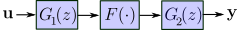
\includegraphics[height=.1\textwidth]{img/dynonet/wiener_hammerstein.pdf}
 %   \end{figure}
 \begin{center}
    model:
    \vskip -2em
    \begin{align*}
    x^+ &=  \mathcal{N}_f(x, u; \theta)\\
    \hat y   &= \mathcal{N}_g(x; \theta)\\
\end{align*}
\end{center}
\column{.66 \textwidth}
 \begin{center}
system: $G_1(z) \Rightarrow F(\cdot) \Rightarrow G_2(z)$
\includegraphics[height=.25\textwidth]{img/uncertainty/WH.pdf}
\end{center}

  \end{columns}
$\mathcal{N}_f, \mathcal{N}_g:$ 1 hidden layer, 15 neurons + linear term, as in \structure{previous literature} \\
\pause
Training on a multisine with std 0.4, bandwidth [0 2] kHz, 10K samples. \\
\pause
 Testing on:
\begin{enumerate}
 \item A multisine with std 0.4, bandwidth [0 2] kHz
 \item A multisine with std 0.4, bandwidth [1 2] kHz
 \item A multisine with std \alert{0.8}, bandwidth [0 2] kHz
 \item A multisine with std 0.4, bandwidth \alert{[0 10]} kHz
 \end{enumerate}
 \pause \vskip .25em
%Training settings from previously published works in this paper\dots
We expect \structure{lower performance and higher uncertainty} on signals 3 and 4.
%The neural network model may fail badly for the test signals 3 and 4. We hope at least to estimate a large uncertainty there!
%\begin
\end{frame}

\begin{frame}{Results: synthetic WH benchmark}
\begin{columns}
\column{.5\textwidth}
\centering
Test signal 1
\includegraphics[width=.9\textwidth]{img/uncertainty/MULTISINE_1.pdf}
\column{.5\textwidth}
\centering
Test signal 2
\includegraphics[width=.9\textwidth]{img/uncertainty/MULTISINE_2.pdf}
\end{columns}

\begin{columns}
\column{.5\textwidth}
\centering
\alert{Test signal 3}
\includegraphics[width=.9\textwidth]{img/uncertainty/MULTISINE_3.pdf}
\column{.5\textwidth}
\centering
\alert{Test signal 4}
\includegraphics[width=.9\textwidth]{img/uncertainty/MULTISINE_4.pdf}
\end{columns}
\structure{Credible intervals} get indeed wider for test signals 3 and 4!
\end{frame}

\begin{frame}{Results: Silverbox benchmark}
Methodology also tested on the original \structure{Silverbox} dataset
\vskip 1em
\begin{columns}
\column{.5\textwidth}
\centering
Test set (full)
\includegraphics[width=.9\textwidth]{img/uncertainty/silverbox.pdf}
\column{.5\textwidth}
\centering
Test set (zoom)
\includegraphics[width=.9\textwidth]{img/uncertainty/silverbox_zoom.pdf}
\end{columns}

\begin{itemize}
 \item Large errors towards the end of the ramp test signal (left plot)
 \item Credible intervals useful, though not calibrated (right plot) 
\end{itemize}
\pause
\vskip 1em
Large values not seen in training, therefore high uncertainty towards the end of the ramp.
\end{frame}


\begin{frame}{Conclusions}{}
\structure{Preliminary} uncertainty quantification for neural state-space models. %The  Uncertainty quantification for neural networks is largely open for research!
\begin{itemize}
 \item In a Bayesian Framework
 \item Using the simplest inference techniques
\end{itemize}
Obtained credible intervals not well calibrated, but allow one to \structure{detect} out-of-distribution regimes.\\
\pause
\vskip 1em
Large room for improvement, both in the theoretical framework and in the approximate inference engine.
\structure{Benchmarks and metrics} also to be devised!
\pause
\vskip 1em
Open opportunity: to exploit the uncertainty for \structure{Experiment Design}!

\end{frame}

\begin{frame}{Bonus topic: Hessian Matrix Analysis}{}
 Wiener-Hammerstein: Hessian matrix at optimum:
 \vskip 1em
 \begin{columns}
 \column{.5\textwidth}
 \centering
 {GN Hessian Matrix abs}
 \includegraphics[width=.9\textwidth]{img/uncertainty/WH_GN_Hessian.png}
 \column{.5\textwidth}
 \centering
 {GN Hessian Matrix eigenvalues}
 \includegraphics[width=.9\textwidth]{img/uncertainty/WH_GN_Hessian_eigs.pdf}
 \end{columns} 
 \vskip 1em
 The Hessian is non-degenerate only in $\sim$ 7 directions. 
\end{frame}

\begin{frame}{Bonus topic: Hessian Matrix Analysis}{}
 Silverbox: Hessian matrix at optimum:
 \vskip 1em
 \begin{columns}
 \column{.5\textwidth}
 \centering
 {GN Hessian Matrix abs}
 \includegraphics[width=.9\textwidth]{img/uncertainty/S_GN_Hessian.png}
 \column{.5\textwidth}
 \centering
 {GN Hessian Matrix eigenvalues}
 \includegraphics[width=.9\textwidth]{img/uncertainty/S_GN_Hessian_eigs.pdf}
 \end{columns} 
 \vskip 1em
 The Hessian is non-degenerate only in $\sim$ 6 directions. 
\end{frame}

% \begin{frame}{}{}
%  The Laplace approximation could be very inaccurate for multimodal
%  posterior distributions.
% \end{frame}

\begin{frame}{}{}
\begin{center}
\huge{\structure{Thank you.\\ Questions?}}\\
\vskip 1em
\begin{small}
\texttt{marco.forgione@idsia.ch}
\end{small}
\end{center}
\end{frame}

\end{document}

\end{document}
